\section{Implementación}\label{sec:implementacion}

\begin{frame}{Diagrama UML}
    \begin{figure}[H]
        \centering
        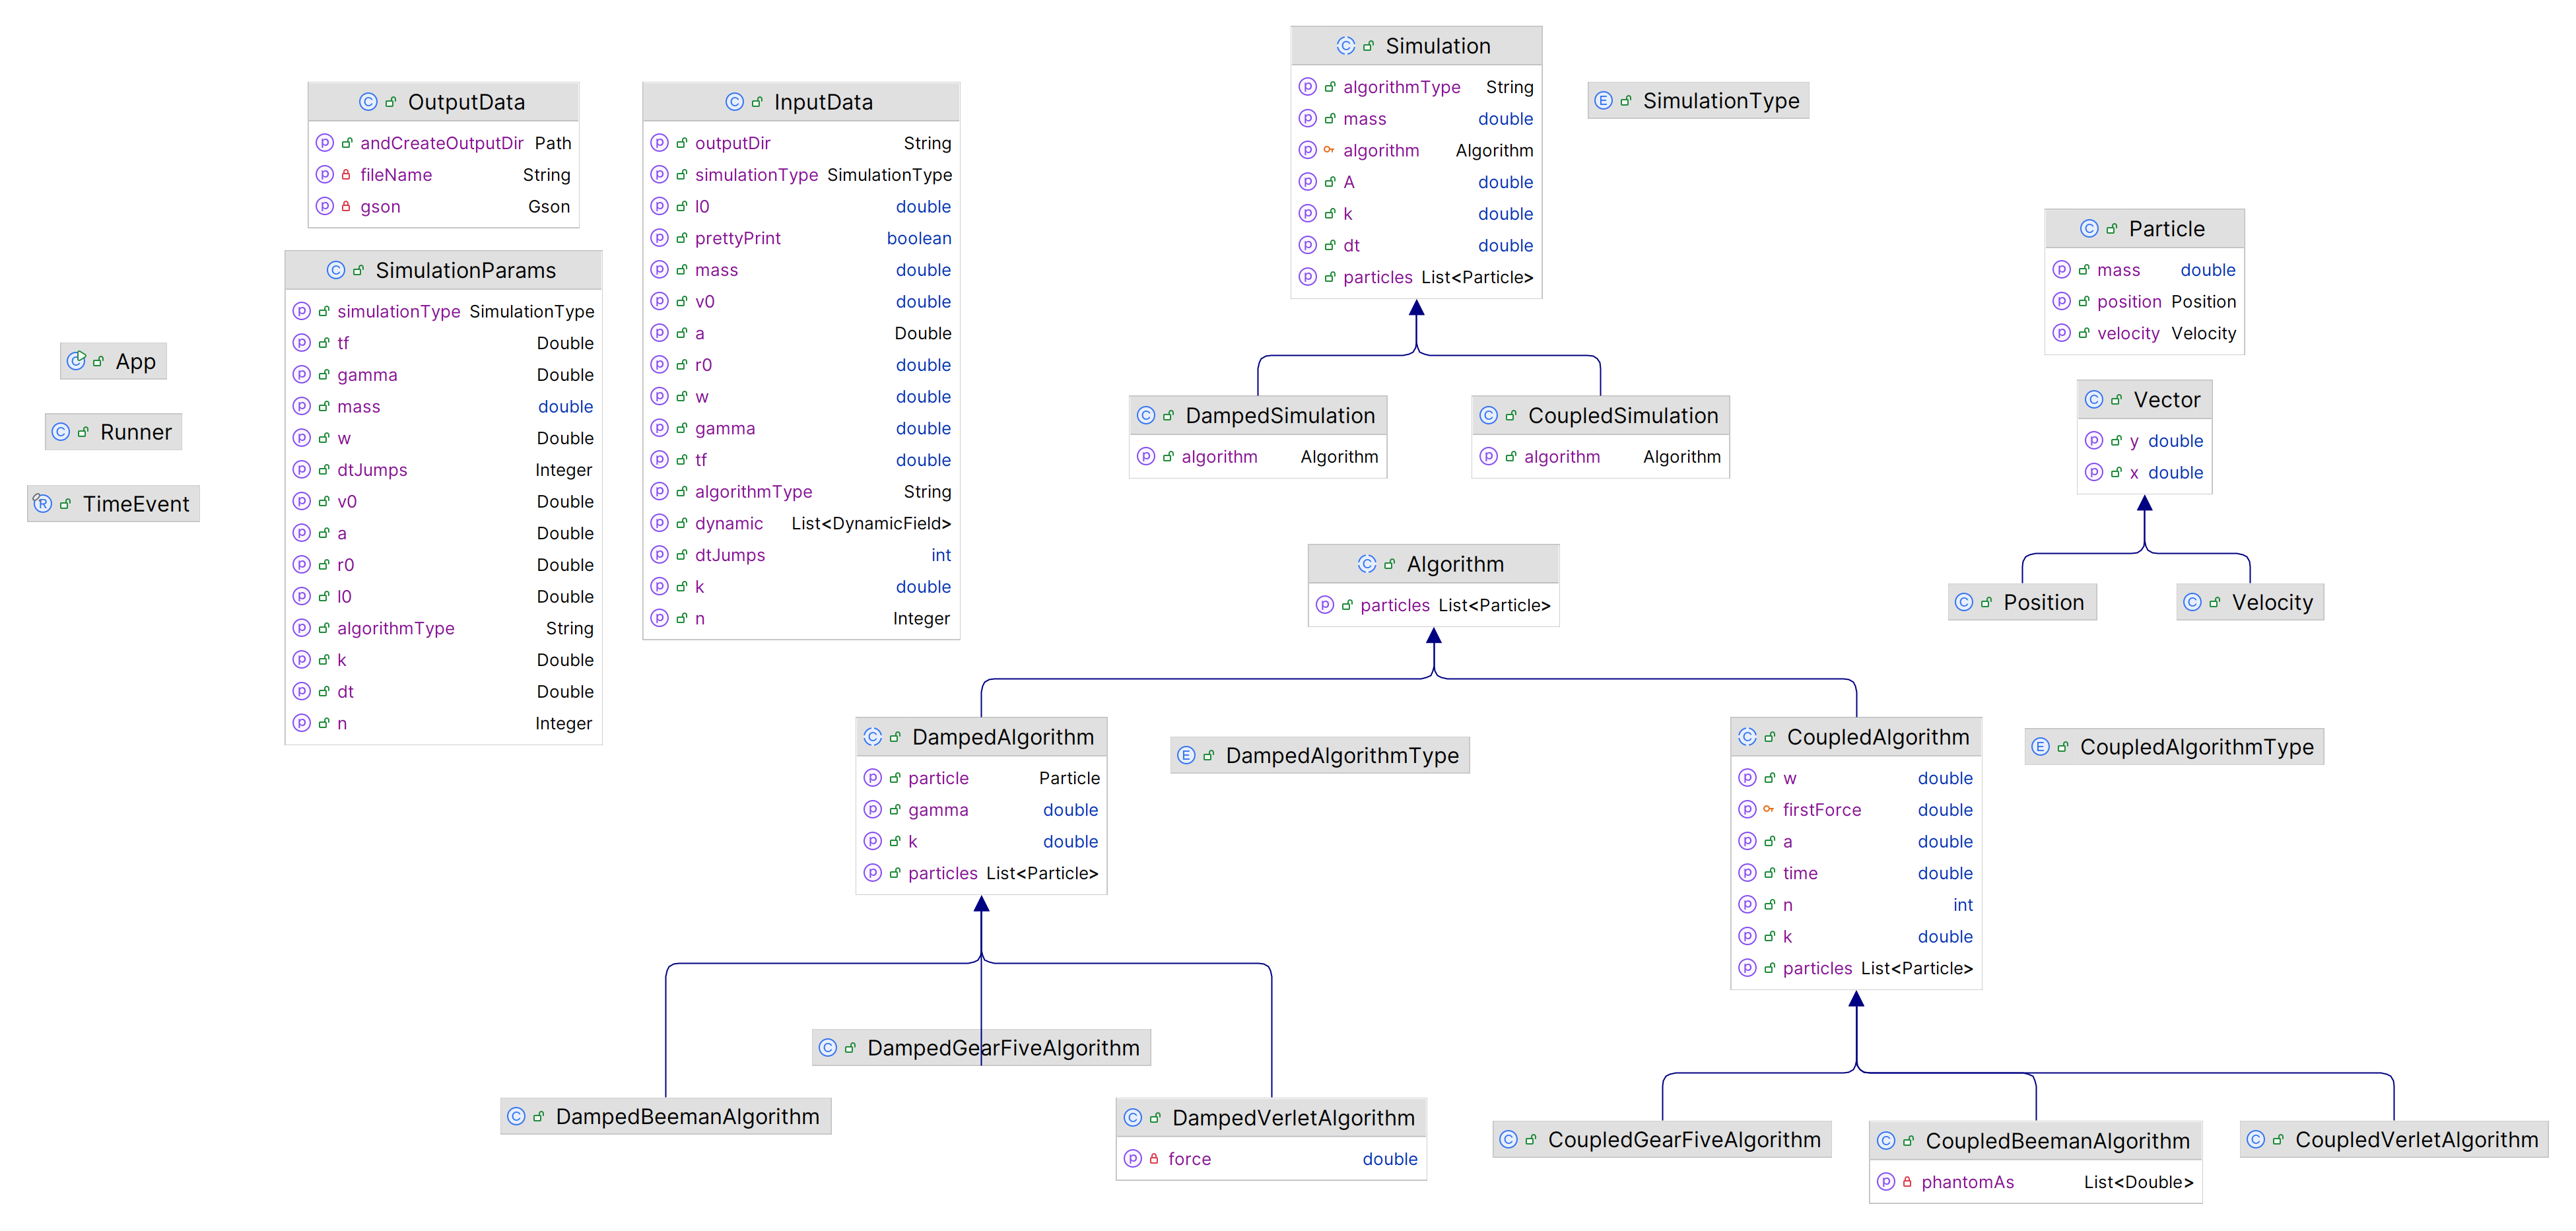
\includegraphics[width=1\linewidth]{pic/03-impl/UML}\label{fig:figure-uml}
    \end{figure}
\end{frame}

\begin{frame}{Pseudocódigo}
    Utilizando Verlet
    \footnotesize{
        \begin{algorithmic}
            \While{\text{$t$ < $t_{max}$}}
                \State \text{Calcular fuerza sobre particula 1}
                \State \text{Calcular fuerzas sobre particulas 2 a N-1}
                \State \text{Actualizar posiciones y velocidades de las particulas 1 a N-1}
                \State \text{Actualizar posicion particula N}
                \State \text{$t \leftarrow \Delta t + t$}
            \EndWhile
        \end{algorithmic}
    }
\end{frame}

